\documentclass[12pt]{article}
\usepackage[left=1in,top=1in,right=1in,bottom=1in]{geometry} 
\geometry{letterpaper} % or letter or a5paper or ... etc
\usepackage{graphicx}
%\usepackage{color}
\usepackage{longtable}


\title{CAMEO Religious Classification System
\thanks{ This framework was developed under the auspices of the Kansas Event Data System project with funding provided by the National Science Foundation SES-0921027 and SES-1004414.}}
\author{Matthias Heilke  }
\date{Version 1.0 : 2011-05-27 \\~\\Updated for the Open Event Data Alliance\\ PLOVER Project: \today} 


\begin{document}

\pagenumbering{gobble} 
\maketitle

\newpage


The comprehensive list of all religious codes is arranged by its subsections as follows: first into named religions, followed by religious categories, each alphabetically arranged; second alphabetically; and third, numerically.  The \LaTeX ~source code for this file can be found at \texttt{https://github.com/openeventdata/PLOVER}.

\begin{figure}[h!]
\centering
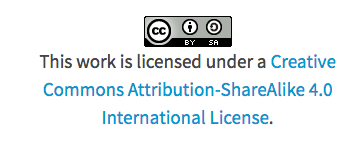
\includegraphics[width=0.6\textwidth]{cc_license}
\end{figure}



\begin{tiny}
\begin{center}
\begin{longtable}{|l|l|}
\caption{Directory of all Religious Codes }
\label{tab:CAMEORCScodes}
\\ \cline{1-1} \cline{1-2}
\textbf{{\normalsize Heirarchical Code}} & \textbf{{\normalsize Religion and Comments }} \\
\hline
\endfirsthead
\hline
\textbf{{\normalsize Heirarchical Code }} & \textbf{{\normalsize Religion and Comments }} \\
\hline
\endhead
\hline
\multicolumn{2}{r}{\emph{Continued on next page}}
\endfoot
\hline
\endlastfoot
\\
{\normalsize REL } & {\normalsize  Unspecified Religious } \\
 \\
{\normalsize ATH } & {\normalsize Agnostic/Atheist } \\
~~ATH010 & Freethought \\
 \\
{\normalsize BAH } & {\normalsize Bahai Faith	~~inc. all non-schismatic Bahai } \\
~~BAH010 & Baha'is Under the Provisions of the Covenant \\
~~BAH020 & Faith of God	~~a.k.a. the House of Mankind and the Universal Palace of Order \\
~~BAH030 & Free Baha'i Faith \\
~~BAH040 & Orthodox Baha'i Faith	~~a.k.a. Mother Baha'i Council \\
~~BAH050 & Orthodox Baha'i Faith Under the Regency \\
~~BAH060 & Charles Mason Remey Society \\
~~BAH070 & The Friends Newsletter \\
 \\
{\normalsize BUD } & {\normalsize Buddhism } \\
~~BUDMAH & Mahayana Buddhism \\
~~~~BUDMAH100 & Pure Land Buddhism	~~a.k.a. Amidism \\
~~~~~~BUDMAH110 & Jodo Shinshu	~~a.k.a. Shin Buddhism \\
~~~~~~~~BUDMAH111 & Hongan-ji School	~~a.k.a. Jodo Shinshu Hompa Hongwanji-ha, Nishi Hongan-ji \\
~~~~~~~~BUDMAH112 & Otani School	~~a.k.a. Jodo Shinshu Otani-ha, Higashi Hongan-ji \\
~~~~~~~~BUDMAH113 & Takada School \\
~~~~~~~~BUDMAH114 & Bukkoji School \\
~~~~~~~~BUDMAH115 & Kosho School \\
~~~~~~~~BUDMAH116 & Kibe School \\
~~~~~~~~BUDMAH117 & Izumoji School \\
~~~~~~~~BUDMAH118 & Joshoji School \\
~~~~~~BUDMAH120 & Jodo Shu	~~(mainline group: "Chinzei" branch) \\
~~~~~~~~BUDMAH121 & Seizan branch \\
~~~~~~BUDMAH130 & Vietnamese Pure Land Buddhism	~~(specifically, Vietnamese Pure Land Buddhism Association) \\
~~~~~~BUDMAH140 & Yuzu Nembutsu \\
~~~~BUDMAH200 & Zen Buddhism	~~a.k.a. Chan Buddhism \\
~~~~~~BUDMAH210 & Classic Zen \\
~~~~~~~~BUDMAH211 & Caodong school	~~inc. Soto sect (Japanese line) \\
~~~~~~~~BUDMAH212 & Fayan school \\
~~~~~~~~BUDMAH213 & Guiyang school \\
~~~~~~~~BUDMAH214 & Linji school	~~inc. Rinzai school (Japanese line) \\
~~~~~~~~BUDMAH215 & Yunmen school \\
~~~~~~BUDMAH220 & Japanese Zen (excluding classical schools) \\
~~~~~~~~BUDMAH221 & Obaku \\
~~~~~~~~BUDMAH223 & Soto \\
~~~~~~BUDMAH230 & Seon Buddhism	~~a.k.a. Korean Zen \\
~~~~~~~~BUDMAH231 & Jogye Order \\
~~~~~~BUDMAH240 & Thien Tong	~~a.k.a. Thien Buddhism, Vietnamese Zen \\
~~~~BUDMAH300 & Nichiren Buddhism	~~(note that a number of names are shared by multiple schools/sects) \\
~~~~~~BUDMAH301 & Fuji Taisekiji Kenshokai \\
~~~~~~BUDMAH302 & Fuju-fuse Nichiren Komon Shu \\
~~~~~~BUDMAH303 & Hokke Nichiren Shu \\
~~~~~~BUDMAH304 & Hokkeshu \\
~~~~~~BUDMAH305 & Hompa Nichiren Shu \\
~~~~~~BUDMAH306 & Honke Nichiren Shu \\
~~~~~~BUDMAH307 & Honmon Butsuryu Shu Ja \\
~~~~~~BUDMAH308 & Honmon Hokke Shu \\
~~~~~~BUDMAH309 & Honmon Kyoo Shu \\
~~~~~~BUDMAH310 & Honmon Shoshu \\
~~~~~~BUDMAH311 & Kempon Hokke Shu \\
~~~~~~BUDMAH312 & Kokuchukai|	~~a.k.a. Kokuchukai ja \\
~~~~~~BUDMAH313 & Nichiren Hokke Shu \\
~~~~~~BUDMAH314 & Nichiren Honshu \\
~~~~~~BUDMAH315 & Nichiren Komon Shu \\
~~~~~~BUDMAH316 & Nichiren Shoshu \\
~~~~~~BUDMAH317 & Nichiren Shu \\
~~~~~~BUDMAH318 & Nichiren Shu Fuju-fuse-ha	~~a.s.a. Nichirenshu Fuju-fuse-ha \\
~~~~~~BUDMAH319 & Nipponzan Myohoji \\
~~~~~~BUDMAH320 & Reiyukai	~~a.k.a. Spiritual-Friendship-Association \\
~~~~~~BUDMAH321 & Rissho Kosei Kai \\
~~~~~~BUDMAH322 & Shobo Hokke Shu \\
~~~~~~BUDMAH323 & Shoshinkai \\
~~~~~~BUDMAH324 & Soka Gakkai \\
~~~~BUDMAH400 & Tiantai and regional variants thereof \\
~~~~~~BUDMAH410 & Cheontae \\
~~~~~~BUDMAH420 & Tendai \\
~~~~BUDMAH500 & Shinnyo-en \\
~~BUDMLN & millenarian Buddhist movements \\
~~~~BUDMLN010 & Aum Shinrikyo	~~a.k.a. Aleph \\
~~~~~~BUDMLN011 & Hikari No Wa \\
~~BUDNRM & new Buddhist movements \\
~~~~BUDNRM010 & Santi Asoke \\
~~BUDSYN & syncretic Buddhism \\
~~~~BUDSYN010 & Tara Center \\
~~BUDTHR & Therevada Buddhism \\
~~~~BUDTHR400 (+500) & Therevada monastic orders \\
~~~~~~BUDTHR410 & Amarapura Nikaya \\
~~~~~~BUDTHR420 & Dhammayuttika Nikaya \\
~~~~~~BUDTHR430 & Dvara Nikaya \\
~~~~~~BUDTHR440 & Maha Nikaya \\
~~~~~~~~BUDTHR441 & Dhammakaya Movement \\
~~~~~~BUDTHR450 & Mahasthabir Nikaya \\
~~~~~~BUDTHR460 & Ramanna Nikaya \\
~~~~~~BUDTHR470 & Sangharaj Nikaya \\
~~~~~~BUDTHR480 & Shwekyin Nikaya \\
~~~~~~BUDTHR490 & Siam Nikaya \\
~~~~~~BUDTHR500 & Thudhamma Nikaya \\
~~BUDVAJ & Vajrayana Buddhism	~~a.k.a. Tantra, Diamond Vehicle, Esoteric Buddhism, … \\
~~~~BUDVAJ100 & Newar Buddhism \\
~~~~BUDVAJ200 & Shingon Buddhism	~~a.k.a. Orthodox Esoteric Buddhism, Japanese Esoteric Buddhism \\
~~~~~~BUDVAJ210 & Kogi Shingon School	~~a.k.a. Ancient Shingon School \\
~~~~~~BUDVAJ220 & Shingi Shingon School	~~a.k.a. Reformed Shingon School \\
~~~~BUDVAJ300 & Shugendo \\
~~~~BUDVAJ400 & Tibetan Buddhism	~~(N.B. all forms of Tibetan Buddhism other than Gelug are called "Red Hat sects") \\
~~~~~~BUDVAJ410 & Gelug	~~a.k.a. Gelug-pa, dGe Lugs Pa, dge-lugs-pa, Dgelugspa, Yellow Hat Sect; includes Dalai Lama \\
~~~~~~BUDVAJ420 & Kagyu	~~a.k.a. Kagyupa, Kagyud \\
~~~~~~~~BUDVAJ421 & Barom Kagyu \\
~~~~~~~~BUDVAJ422 & Drubgyu Karma Kamtsang	~~a.k.a. Karma Kagyu, Karma Kamtsang, Karmapa Sect \\
~~~~~~~~BUDVAJ423 & Drikung Kagyu \\
~~~~~~~~BUDVAJ424 & Drukpa Kagyu \\
~~~~~~~~BUDVAJ425 & Shangpa Kagyu \\
~~~~~~~~BUDVAJ426 & Taklung Kagyu \\
~~~~~~BUDVAJ430 & Nyingma	~~a.k.a. Nyingmapa \\
~~~~~~BUDVAJ440 & Rime Movement	~~(ecumenical/"eclectic" movement) \\
~~~~~~BUDVAJ450 & Sakya	~~a.k.a. Sakyapa \\
~~~~~~~~BUDVAJ451 & Ngor \\
~~~~~~~~BUDVAJ452 & Tshar \\
 \\
{\normalsize CHR } & {\normalsize Christianity } \\
~~CHR001 & Charismatic Christianity \\
~~CHR002 & conservative Christianity \\
~~CHR003 & evangelical Christianity \\
~~CHR004 & liberal Christianity \\
~~CHR005 & Prosperity theology \\
~~CHR100 & ecumenical Christian movements \\
~~~~CHR101 & World Council of Churches \\
~~CHRANG & Anglican Communion \\
~~~~~~CHRANG001 & Anglican \\
~~~~~~CHRANG002 & Episcopalian \\
~~~~~~CHRANG011 & "conservative" Anglican \\
~~~~~~CHRANG012 & "liberal" Anglican \\
~~~~~~CHRANG013 & "high" Anglican \\
~~~~~~CHRANG014 & "low" Anglican \\
~~~~~~CHRANG015 & "Catholic" Anglican \\
~~~~CHRANG900 & schismatic Catholics within the Anglican Communion \\
~~~~~~CHRANG901 & Philippine Independent Church \\
~~~~~~CHRANG902 & (Old Catholic Church	~~inc. Union of Utrech and any other Old Catholic members of the Anglican Communion) \\
~~CHRCTH & Roman Catholic	~~	~~(Latin Rite is defined as the mainstream) \\
~~~~CHRCTH001 & Liberation Theology \\
~~~~CHRCTH200 (+300) & Roman Catholic laity \\
~~~~~~CHRCTH201 & Apostolate for Family Consecration \\
~~~~~~CHRCTH202 & Catholic Charismatic Renewal \\
~~~~~~CHRCTH203 & Catholic Worker Movement \\
~~~~~~CHRCTH204 & Communion and Liberation \\
~~~~~~CHRCTH205 & Community of Sant'Egidio \\
~~~~~~CHRCTH206 & Cursillo Movement \\
~~~~~~CHRCTH207 & Focolare Movement \\
~~~~~~CHRCTH208 & L'Arche \\
~~~~~~CHRCTH209 & Legion of Mary \\
~~~~~~CHRCTH210 & Madonna House Apostolate \\
~~~~~~CHRCTH211 & Neocatechumenal Way \\
~~~~~~CHRCTH212 & Regnum Christi \\
~~~~~~CHRCTH213 & Schoenstatt Movement \\
~~~~~~CHRCTH214 & Worldwide Marriage \\
~~~~CHRCTH400 (+500) & Roman Catholic monastic orders \\
~~~~~~CHRCTH401 & Adorers 	~~a.k.a. Adorers of the Blood of Christ \\
~~~~~~CHRCTH402 & Adornos 	~~a.k.a. Clerics Regular Minor \\
~~~~~~CHRCTH403 & Assumptionists 	~~a.k.a. Augustinians of the Assumption \\
~~~~~~CHRCTH404 & Society of the Atonement 	~~a.k.a. Atonement Friars/Graymoor Friars/Sisters \\
~~~~~~CHRCTH405 & Augustinians 	~~a.k.a. Order of Saint Augustine \\
~~~~~~CHRCTH406 & Baladites 	~~a.k.a. Order of Lebanese Maronite \\
~~~~~~CHRCTH407 & Barnabites 	~~a.k.a. Clerics Regular of Saint Paul \\
~~~~~~CHRCTH408 & Basilians 	~~a.k.a. Congregation of St. Basil \\
~~~~~~CHRCTH409 & Benedictines 	~~a.k.a. Order of Saint Benedict \\
~~~~~~CHRCTH410 & Bridgettines 	~~a.k.a. Order of Our Savior \\
~~~~~~CHRCTH411 & Brothers of Christian Instruction of St Gabriel \\
~~~~~~CHRCTH412 & Brothers of the Christian Schools 	~~a.k.a. Lasallian Brothers or Christian Brothers \\
~~~~~~CHRCTH413 & Brothers of Mercy of Our Lady of Perpetual Help \\
~~~~~~CHRCTH414 & Camaldolese 	~~a.k.a. Camaldolese Benedictines \\
~~~~~~CHRCTH415 & Camillians 	~~a.k.a. Order of Saint Camillus \\
~~~~~~CHRCTH416 & Canossians 	~~a.k.a. Canossian Daughters and Sons of Charity \\
~~~~~~CHRCTH417 & Canons Regular of the New Jerusalem \\
~~~~~~CHRCTH418 & Capuchins 	~~a.k.a. Order of Friars Minor Capuchin \\
~~~~~~CHRCTH419 & Carmelites 	~~a.k.a. Order of Our Lady of Mt. Carmel \\
~~~~~~CHRCTH420 & Carmelites of Mary Immaculate \\
~~~~~~CHRCTH421 & Carthusians \\
~~~~~~CHRCTH422 & Celestines 	~~defunct \\
~~~~~~CHRCTH423 & Cistercians \\
~~~~~~CHRCTH424 & Claretians 	~~a.k.a. Claretian Missionaries \\
~~~~~~CHRCTH425 & Columbans 	~~a.k.a. Missionary Society of St. Columban \\
~~~~~~CHRCTH426 & Congregatio Immaculatae Cordis Mariae 	~~a.k.a. Scheutfathers, Scheutists, Missionhurst \\
~~~~~~CHRCTH427 & Congregation of the Disciples of the Lord \\
~~~~~~CHRCTH428 & Congregation of Holy Cross \\
~~~~~~CHRCTH429 & Congregation of Notre Dame \\
~~~~~~CHRCTH430 & Congregation of the Sacred Hearts of Jesus and Mary \\
~~~~~~CHRCTH431 & Conventual Franciscans 	~~a.k.a. Conventuals or Order of Friars Minor Conventual \\
~~~~~~CHRCTH432 & Crosiers 	~~a.k.a. Canons Regular of the Holy Cross \\
~~~~~~CHRCTH433 & Daughters of Charity of St. Vincent de Paul \\
~~~~~~CHRCTH434 & Dehonians 	~~a.k.a. Priests of the Sacred Heart of Jesus \\
~~~~~~CHRCTH435 & Divine Word Missionaries \\
~~~~~~CHRCTH436 & Discalced Carmelites \\
~~~~~~CHRCTH437 & Dominicans 	~~a.k.a. Order of Friars Preachers \\
~~~~~~CHRCTH438 & Dottrinari 	~~a.k.a. Congregazione dei Preti della Dottrina Cristiana \\
~~~~~~CHRCTH439 & Eudists 	~~a.k.a. Congregation of Jesus and Mary \\
~~~~~~CHRCTH440 & Franciscan Brothers of Brooklyn \\
~~~~~~CHRCTH441 & Franciscans 	~~a.k.a. Order of Friars Minor \\
~~~~~~CHRCTH442 & Franciscan Missionaries of Divine Motherhood \\
~~~~~~CHRCTH443 & Franciscan Missionaries of Mary \\
~~~~~~CHRCTH444 & Franciscan Friars of the Third Order Regular \\
~~~~~~CHRCTH445 & Fransalians 	~~a.k.a. Missionaries of St. Francis de Sales \\
~~~~~~CHRCTH446 & Grey Nuns of the Sacred Heart \\
~~~~~~CHRCTH447 & Good Shepherd Sisters \\
~~~~~~CHRCTH448 & Handmaids of the Blessed Sacrament and of Charity \\
~~~~~~CHRCTH449 & Handmaids of the Sacred Heart of Jesus \\
~~~~~~CHRCTH450 & Holy Cross Fathers 	~~a.k.a. Congregation of Holy Cross \\
~~~~~~CHRCTH451 & Order of Hospitalers 	~~a.k.a. Hospitaler Brothers of St. John of God \\
~~~~~~CHRCTH452 & Infant Jesus Sisters 	~~a.k.a. Nicolas Barre \\
~~~~~~CHRCTH453 & Institute of Christ the King Sovereign Priest \\
~~~~~~CHRCTH454 & Jesuits 	~~a.k.a. Society of Jesus \\
~~~~~~CHRCTH455 & Josephines of Asti 	~~a.k.a. Oblates of St. Joseph \\
~~~~~~CHRCTH456 & Josephite Fathers and Brothers 	~~a.k.a. St. Joseph's Society of the Sacred Heart \\
~~~~~~CHRCTH457 & Lazarists 	~~a.k.a. Vincentians, Congregation of the Mission \\
~~~~~~CHRCTH458 & Legionaries of Christ \\
~~~~~~CHRCTH459 & Little Sisters of the Poor \\
~~~~~~CHRCTH460 & Loreto Sisters 	~~a.k.a. Institute of the Blessed Virgin Mary \\
~~~~~~CHRCTH461 & Marian Fathers \\
~~~~~~CHRCTH462 & Marianists 	~~a.k.a. Marists, Daughters of Mary Immaculate, Society of Mary \\
~~~~~~CHRCTH465 & Marist Brothers \\
~~~~~~CHRCTH466 & Maryknoll 	~~a.k.a. Catholic Foreign Mission Society of America \\
~~~~~~CHRCTH467 & Mercedarians 	~~a.k.a. Order of Our Lady of Mercy \\
~~~~~~CHRCTH468 & Missionaries of Charity \\
~~~~~~CHRCTH469 & Missionaries of the Sacred Heart \\
~~~~~~CHRCTH470 & Missionary Contemplative Movement "P. de Foucauld"	~~a.k.a. Centro Missionario "P. de Foucauld" \\
~~~~~~CHRCTH471 & Norbertines or Premonstratensians 	~~a.k.a. Canons Regular of Prémontré \\
~~~~~~CHRCTH472 & Olivetans 	~~a.k.a. Order of Our Lady of Mount Olivet \\
~~~~~~CHRCTH473 & Oblates Of Mary Immaculate \\
~~~~~~CHRCTH474 & Oblate Sisters of Providence \\
~~~~~~CHRCTH475 & Oratorians 	~~a.k.a. Oratory of St. Philip Neri \\
~~~~~~CHRCTH476 & Order of St. Elisabeth \\
~~~~~~CHRCTH477 & Pallottines 	~~a.k.a. Society of the Catholic Apostolate \\
~~~~~~CHRCTH478 & Paris Foreign Missions Society 	~~a.k.a. Missions Etrangères de Paris \\
~~~~~~CHRCTH479 & Passionists	~~a.k.a. Congregation of the Passion \\
~~~~~~CHRCTH480 & Paulists 	~~a.k.a. Congregation of St. Paul \\
~~~~~~CHRCTH481 & Piarists 	~~a.k.a. Clerics Regulars Poors of the Mother of God of the Pious Schools \\
~~~~~~CHRCTH482 & Poor Clares 	~~a.k.a. Nuns of the Order of St. Clare/(Order of Poor Ladies \\
~~~~~~CHRCTH483 & Presentation Brothers \\
~~~~~~CHRCTH484 & Presentation Sisters	~~a.k.a. Sisters of the Presentation of the Blessed Virgin Mary \\
~~~~~~CHRCTH485 & Priestly Fraternity of St. Peter \\
~~~~~~CHRCTH486 & Redemptorists 	~~a.k.a. Congregation of the Most Holy Redeemer \\
~~~~~~CHRCTH487 & Religious of the Cenacle \\
~~~~~~CHRCTH488 & Resurrectionists \\
~~~~~~CHRCTH489 & Rogationists of the Heart of Jesus \\
~~~~~~CHRCTH490 & Rosminians 	~~a.k.a. Institute of Charity \\
~~~~~~CHRCTH491 & Sacramentines 	~~a.k.a. Congregation of the Blessed Sacrament \\
~~~~~~CHRCTH492 & Salesians of St. John Bosco	~~a.k.a. Salesian Society, Salesians of John Bosco, Society of St. Francis de Sales \\
~~~~~~CHRCTH493 & Salesian Sisters 	~~a.k.a. Daughters of Mary Help of Christian, (Daughters of St. Francis de Sales?) \\
~~~~~~CHRCTH494 & Salvatorians 	~~a.k.a. Society of the Divine Savior \\
~~~~~~CHRCTH495 & Scalabrians 	~~a.k.a. Congregation of the Missionaries of St. Charles Borromeo \\
~~~~~~CHRCTH496 & School Sisters of Notre Dame \\
~~~~~~CHRCTH497 & Servites 	~~a.k.a. Order of Friars, Servants of Mary \\
~~~~~~CHRCTH498 & Sisters of Charity \\
~~~~~~CHRCTH499 & Sisters of Charity of the Blessed Virgin Mary \\
~~~~~~CHRCTH500 & Sisters of the Holy Names of Jesus and Mary \\
~~~~~~CHRCTH501 & Sisters of Mercy or Religious Sisters of Mercy \\
~~~~~~CHRCTH502 & Sisters of Notre Dame de Namur \\
~~~~~~CHRCTH503 & Sisters of Our Lady of Mercy \\
~~~~~~CHRCTH504 & Sisters of St Joseph \\
~~~~~~CHRCTH505 & Sisters of St Joseph of the Sacred Heart \\
~~~~~~CHRCTH506 & Society of the Precious Blood 	~~a.k.a. Precious Blood Fathers \\
~~~~~~CHRCTH507 & Spiritans or Holy Ghost Fathers 	~~a.k.a. Congregation of the Holy Ghost \\
~~~~~~CHRCTH508 & Stigmatines 	~~a.k.a. Congregation of the Sacred Stigmata \\
~~~~~~CHRCTH509 & Sulpician Fathers 	~~a.k.a. Society of Saint Sulpice \\
~~~~~~CHRCTH510 & Theatines 	~~a.k.a. Congregation of Clerics Regular \\
~~~~~~CHRCTH511 & Trappists 	~~a.k.a. Order of Cistercians of the Strict Observance \\
~~~~~~CHRCTH512 & Trinitarians 	~~a.k.a. Order of the Most Holy Trinity \\
~~~~~~CHRCTH513 & Ursulines 	~~a.k.a. Ursuline Nuns of the Roman Union, also Ursuline Sisters of Tildonck \\
~~~~~~CHRCTH514 & Verbum Dei Missionary Fraternity \\
~~~~~~CHRCTH515 & Viatorians 	~~a.k.a. Clerics of Saint Viator \\
~~~~~~CHRCTH517 & Vocationists 	~~a.k.a. Clerics of the Divine Vocation \\
~~~~~~CHRCTH518 & Xaverians or Xaverian Brothers 	~~a.k.a. Missionary Society of St. Francis Xavier \\
~~~~CHRCTH600 & miscellaneous Roman Catholic organizations \\
~~~~~~CHRCTH601 & Opus Dei \\
~~~~~~CHRCTH602 & personal ordinariates of former Anglicans \\
~~~~~~CHRCTH603 & Sovereign Military Hospitaller Order of Saint John of Jerusalem of Rhodes and of Malta	~~a.k.a. Order of Malta \\
~~~~CHRCTH800 & Eastern Catholic Church \\
~~~~~~CHRCTH810 & Alexandrian liturgical tradition \\
~~~~~~~~CHRCTH811 & Coptic Catholic Church \\
~~~~~~~~CHRCTH812 & Ethiopian Catholic Church \\
~~~~~~CHRCTH820 & Antiochan liturgical tradition \\
~~~~~~~~CHRMRN & Maronite Church	~~(could also call it "CHRCTH921") \\
~~~~~~~~CHRCTH822 & Syriac Catholic Church \\
~~~~~~~~CHRCTH823 & Syro-Malankara Catholic Church \\
~~~~~~CHRCTH830 & Armenian liturgical tradition \\
~~~~~~~~CHRCTH831 & Armenian Catholic Church \\
~~~~~~CHRCTH840 & Chaldean/East Syrian liturgical tradition \\
~~~~~~~~CHRCTH841 & Chaldean Catholic Church \\
~~~~~~~~CHRCTH842 & Syro-Malabar Church \\
~~~~~~CHRCTH850 (+860) & Byzantine liturgical tradition \\
~~~~~~~~CHRCTH851 & Albanian Catholic Church \\
~~~~~~~~CHRCTH852 & Belarusian Catholic Church \\
~~~~~~~~CHRCTH853 & Bulgarian Catholic Church \\
~~~~~~~~CHRCTH854 & Eparchy of Krizevci \\
~~~~~~~~CHRCTH855 & Eucharistic Catholic Church \\
~~~~~~~~CHRCTH856 & Greek Byzantine Catholic Church \\
~~~~~~~~CHRCTH857 & Hungarian Catholic Church \\
~~~~~~~~CHRCTH858 & Italo-Albanian Catholic Church \\
~~~~~~~~CHRCTH859 & Macedonian Catholic Church \\
~~~~~~~~CHRCTH860 & Melkite Greek Catholic Church \\
~~~~~~~~CHRCTH861 & Romanian Church United with Rome \\
~~~~~~~~CHRCTH862 & Russian Catholic Church \\
~~~~~~~~CHRCTH863 & Ruthenian Catholic Church \\
~~~~~~~~CHRCTH864 & Slovak Catholic Church \\
~~~~~~~~CHRCTH865 & Ukrainian Catholic Church \\
~~~~CHRCTH900 & schismatic Catholics \\
~~~~~~CHRCTH901 & African Church Incorporated \\
~~~~~~CHRCTH902 & Antiochian Catholic Church in America	~~(we can reserve the 100's for Catholic schisms) \\
~~~~~~CHRCTH903 & Worldwide Communion of Catholic Apostolic Churches	~~(led by Brazilian Catholic Apostolic Church) \\
~~~~~~CHRCTH904 & Chinese Patriotic Catholic Association \\
~~~~~~CHRCTH905 & Heenum Catholic Church \\
~~~~~~CHRCTH906 & Independent Catholic Churches \\
~~~~~~CHRCTH907 & Liberal Catholic Church \\
~~~~~~CHRCTH908 & Mariavite Church \\
~~~~~~CHRCTH909 & Polish National Catholic Church	~~(and Polish Catholic Church) \\
~~~~~~CHRCTH910 & Society of Saint Pius X \\
~~CHRDOX & Orthodox Christian	~~(Note: category includes all non-Catholic forms of "Eastern" Christianity) \\
~~~~CHRDOX100 & Orthodox Communion	~~(listed in order of seniority, rather than alphabetized) \\
~~~~~~CHRDOX101 & Ecumenical Patriarchate of Constantinople \\
~~~~~~CHRDOX102 & Orthodox Church of Alexandria \\
~~~~~~CHRDOX103 & Orthodox Church of Antioch \\
~~~~~~CHRDOX104 & Orthodox Church of Jerusalem \\
~~~~~~CHRDOX105 & Orthodox Church of Russia \\
~~~~~~CHRDOX106 & Orthodox Church of Serbia \\
~~~~~~CHRDOX107 & Orthodox Church of Romania \\
~~~~~~CHRDOX108 & Orthodox Church of Bulgaria \\
~~~~~~CHRDOX109 & Orthodox Church of Georgia \\
~~~~~~CHRDOX110 & Orthodox Church of Cyprus \\
~~~~~~CHRDOX111 & Orthodox Church of Greece \\
~~~~~~CHRDOX112 & Orthodox Church of Poland \\
~~~~~~CHRDOX113 & Orthodox Church of Albania \\
~~~~~~CHRDOX114 & Orthodox Church of the Czech lands and Slovakia \\
~~~~~~CHRDOX115 & Orthodox Church in America \\
~~~~CHRDOX200 & autonomous, unrecognized, and separated Orthodox \\
~~~~~~CHRDOX201 & American World Patriarchs \\
~~~~~~CHRDOX202 & Belarusian Autocephalous Orthodox Church \\
~~~~~~CHRDOX203 & Chinese Orthodox Church \\
~~~~~~CHRDOX204 & Croatian Orthodox Church \\
~~~~~~CHRDOX205 & Estonian Orthodox Church \\
~~~~~~CHRDOX206 & Finnish Orthodox Church \\
~~~~~~CHRDOX207 & Greek Old Calendarists \\
~~~~~~CHRDOX208 & Japanese Orthodox Church \\
~~~~~~CHRDOX209 & Latvian Orthodox Church \\
~~~~~~CHRDOX210 & Macedonian Orthodox Church \\
~~~~~~CHRDOX211 & Metropolitan Church of Bessarabia \\
~~~~~~CHRDOX212 & Moldovan Orthodox Church \\
~~~~~~CHRDOX213 & Montenegrin Orthodox Church \\
~~~~~~CHRDOX214 & Old Believers \\
~~~~~~CHRDOX215 & Old Calendar Bulgarian Orthodox Church \\
~~~~~~CHRDOX216 & Old Calendar Romanian Orthodox Church \\
~~~~~~CHRDOX217 & Orthodox Church in Italy \\
~~~~~~CHRDOX218 & Orthodox Church of Greece (Holy Synod in Resistance) \\
~~~~~~CHRDOX219 & Orthodox Ohrid Archbishopric \\
~~~~~~CHRDOX220 & Patriarchal Exarchate in Western Europe \\
~~~~~~CHRDOX221 & Russian Orthodox Church Outside Russia \\
~~~~~~CHRDOX222 & Russian True Orthodox Church \\
~~~~~~CHRDOX223 & Ukrainian Orthodox Church (Kyiv Patriarchate) \\
~~~~~~CHRDOX224 & Ukrainian Orthodox Church (Moscow Patriarchate) \\
~~~~CHRDOX300 & Oriental Orthodox	~~Oriental Orthodox \\
~~~~~~CHRDOX301 & Armenian Apostolic Church \\
~~~~~~CHRCPT & Coptic Orthodox	~~(could also call it "CHRDOX202") \\
~~~~~~CHRDOX303 & Eritrean Orthodox \\
~~~~~~CHRDOX304 & Ethiopian Orthodox \\
~~~~~~CHRDOX305 & Malankara Orthodox Syrian Church	~~(also known as Indian Orthodox) \\
~~~~~~CHRDOX306 & Syriac Orthodox \\
~~~~CHRDOX400 & Assyrian Church of the East \\
~~~~CHRDOX500 & Ancient Church of the East \\
~~~~CHRDOX900 & schismatic Orthodox \\
~~~~~~CHRDOX910 & Old Believers - Bespopovtsy \\
~~~~~~~~CHRDOX911 & Pomortsy	~~a.k.a. Danilovtsy \\
~~~~~~~~CHRDOX912 & Novopomortsy	~~a.k.a. New Pomortsy \\
~~~~~~~~CHRDOX913 & Staropomortsy	~~a.k.a. Old Pomortsy \\
~~~~~~~~CHRDOX914 & Fedoseevtsy	~~a.k.a. Society of Christian Old Believers of the Old Pomortsy Unmarried Confession \\
~~~~~~~~CHRDOX915 & Fillipovtsy \\
~~~~~~~~CHRDOX916 & Chasovennye	~~a.k.a. Semeyskie \\
~~~~~~CHRDOX920 & Old Believers - Popovtsy \\
~~~~~~~~CHRDOX921 & Belokrinitskaya hierarchy	~~a.k.a. Russian Orthodox Old-Rite Church \\
~~~~~~~~CHRDOX922 & Novozybkovskaya hierarchy	~~a.k.a. Russian Old-Orthodox Church \\
~~CHRGNO & gnostic Christianity \\
~~~~CHRGNO010 & Anthroposophy \\
~~~~CHRGNO020 & Foundation for Inner Peace	~~i.e. A Course in Miracles \\
~~~~CHRGNO030 & Order of the Solar Temple \\
~~~~CHRGNO040 (041-059) & Rosecrucianism	~~(maybe? Esoteric knowledge ≠ Gnosticism?) \\
~~~~~~CHRGNO041 & Ancient Mystical Order Rosae Crucis \\
~~~~~~CHRGNO042 & Antiquus Ordo Rosicrucianis	~~a.k.a. Ancient Order of the Rosicrucians \\
~~~~~~CHRGNO043 & Fraternitas Rosae Crucis \\
~~~~~~CHRGNO044 & Lectorium Rosicrucianum \\
~~~~~~CHRGNO045 & Rosicrucian Fellowship \\
~~~~~~CHRGNO046 & Societas Rosicruciana \\
~~~~CHRGNO060 & Summum \\
~~CHRJHW & Bible Student Movement	~~(mainline group: Jehovah's Witnesses) \\
~~~~CHRJHW010 & Chicago Bible Students \\
~~~~CHRJHW020 & Christian Millennial Fellowship \\
~~~~CHRJHW030 & Dawn Bible Students \\
~~~~CHRJHW040 & Free Bible Students \\
~~~~~~CHRJHW041 & Berean Bible Students Church \\
~~~~~~CHRJHW042 & Christian Millennial Fellowship	~~a.k.a. Free Bible Students \\
~~~~CHRJHW050 & Friends of Man	~~a.k.a. Philanthropic Assembly of the Friends of Man, The Church of the Kingdom of God \\
~~~~CHRJHW070 & Goshen Fellowship \\
~~~~CHRJHW080 & Independent Bible Students \\
~~~~CHRJHW090 & Laymen's Home Missionary Movement	~~hostile to JW church \\
~~~~CHRJHW100 & True Faith Jehovah's Witnesses Association \\
~~CHRLDS & Latter Day Saints	~~a.k.a. Mormonism \\
~~~~CHRLDS010 & Aaronic Order	~~numbering — Aaronic Order isn't mainstream, right? \\
~~~~CHRLDS020 & Church of Christ (Temple Lot) \\
~~~~CHRLDS030 & Church of Christ with the Elijah Message \\
~~~~CHRLDS040 & Church of the Firstborn of the Fulness of Times \\
~~~~CHRLDS050 & Church of the Lamb of God \\
~~~~CHRLDS060 & Community of Christ	~~a.k.a. Reorganized Church of Jesus Christ of Latter Day Saints \\
~~~~~~CHRLDS061 & Restoration Branches \\
~~~~CHRLDS070 & Confederate Nations of Israel \\
~~~~CHRLDS080 & Fundamentalist Church of Jesus Christ of Latter Day Saints	~~a.k.a. FLDS \\
~~~~CHRLDS090 & Latter-day Church of Christ	~~a.k.a. Kingston Clan, Kingston Group, Davis County Cooperative, The Co-op Society \\
~~~~CHRLDS100 & Rigdonites \\
~~~~CHRLDS110 & Righteous Branch of the Church of Jesus Christ of Latter-day Saints \\
~~~~CHRLDS120 & The Church of Jesus Christ (Bickertonite) \\
~~~~CHRLDS130 & The Church of Jesus Christ of Latter Day Saints (Strangite) \\
~~~~CHRLDS140 & Zion's Order \\
~~CHRMAY & "maybe" Christian — churches of controversial status \\
~~~~CHRMAY001 & esoteric Christianity \\
~~~~CHRMAY110 (111-139) & Armstrongism	~~(the "mainline" group is Grace Communion International) \\
~~~~~~CHRMAY111 & Christian Churches of God \\
~~~~~~CHRMAY112 & Christian Educational Ministries \\
~~~~~~CHRMAY113 & Church of God, 21st Century \\
~~~~~~CHRMAY114 & Church of God, an International Community \\
~~~~~~CHRMAY115 & Church of God International (USA) \\
~~~~~~CHRMAY116 & Church of God, The Eternal \\
~~~~~~CHRMAY117 & Church of God Preparing for the Kingdom of God \\
~~~~~~CHRMAY118 & Church of the Eternal God \\
~~~~~~CHRMAY119 & Church of the Great God \\
~~~~~~CHRMAY120 & Global Church of God (and offshoots) \\
~~~~~~CHRMAY121 & Intercontinental Church of God \\
~~~~~~CHRMAY122 & Living Church of God \\
~~~~~~CHRMAY123 & Philadelphia Church of God \\
~~~~~~CHRMAY124 & Restored Church of God \\
~~~~~~CHRMAY125 & Church of God Fellowship \\
~~~~~~CHRMAY126 & Church of the Great God \\
~~~~~~CHRMAY127 & Sabbath Church of God \\
~~~~~~CHRMAY128 & United Church of God \\
~~~~CHRMAY120 & Assemblies of Yahweh \\
~~~~CHRMAY130 & Bethel Ministerial Association \\
~~~~CHRMAY140 & Christadelphianism	~~a.k.a. Thomasites \\
~~~~CHRMAY150 & Christian Conventions	~~a.k.a. Two-by-Twos, the Workers and Friends \\
~~~~~~CHRMAY151 & Cooneyites \\
~~~~CHRMAY160 & Christian Science	~~a.k.a. Church of Christ, Scientist \\
~~~~CHRMAY170 & Church of the Blessed Hope \\
~~~~CHRMAY180 & Friends of Man \\
~~~~CHRMAY190 & Iglesia ni Cristo \\
~~~~CHRMAY200 & The Local Church	~~a.k.a. Little Flock \\
~~~~CHRMAY210 & Members Church of God International \\
~~~~CHRMAY220 & Mita Congregation \\
~~~~CHRMAY230 & New Thought Movement	~~inc. only the Christian, official New Thought movements \\
~~~~~~CHRMAY231 & Church of Divine Science \\
~~~~~~CHRMAY232 & Religious Science \\
~~~~~~CHRMAY233 & Unity School of Christianity	~~a.k.a. Unity Church \\
~~~~CHRMAY240 & Oneness Pentecostalism	~~(maybe delete some members \\
~~~~~~CHRMAY241 & United Pentecostal Church International \\
~~~~~~CHRMAY242 & Pentecostal Assemblies of the World \\
~~~~CHRMAY250 & Spiritual Christianity \\
~~~~~~CHRMAY251 & Molokans \\
~~~~~~CHRMAY252 & Dukhobors	~~a.s.a. Doukhobors \\
~~~~~~CHRMAY253 & Khlysts \\
~~~~~~CHRMAY254 & Skoptsy \\
~~~~~~CHRMAY255 & Ikonobortsy \\
~~~~CHRMAY260 & Swedenborgianism	~~a.k.a. The Lord's New Church, Church of the New Jerusalem \\
~~~~CHRMAY270 & The Way International \\
~~~~~~CHRMAY271 & American Fellowship Services \\
~~~~~~CHRMAY272 & Great Lakes Fellowship \\
~~~~~~CHRMAY273 & Pacific West Fellowship \\
~~~~CHRMAY280 & Unification Church (Moonies) \\
~~CHRMLN & millenarian Christianity \\
~~~~CHRMLN010 & Branch Davidians \\
~~~~CHRMLN020 & The Brethren	~~a.k.a. The Body of Christ, The Garbage Eaters \\
~~~~CHRMLN030 & Concerned Christians \\
~~CHRNRM & new Christian movements \\
~~~~CHRNRM010 & The Body of Christ \\
~~~~CHRNRM020 & Church of the Living Word	~~a.k.a. The Walk \\
~~~~CHRNRM030 & The Family International \\
~~~~CHRNRM040 & Foundation of Human Understanding \\
~~~~CHRNRM050 & International Community of Christ \\
~~~~CHRNRM060 & Shepherding Movement \\
~~CHROFF & offshoots of Christianity \\
~~~~CHROFF010 & National Spiritualist Association of Churches \\
~~~~CHROFF020 & Spiritualism \\
~~~~CHROFF030 & Unitarian-Universalism \\
~~~~~~CHROFF031 & Covenant of Unitarian Universalist Pagans \\
~~~~~~CHROFF032 & Unitarianism \\
~~~~~~CHROFF033 & Universalism \\
~~~~CHROFF040 & Urantia Foundation \\
~~CHRPRO & Protestant \\
~~~~CHRPRO010 & (Protestant - generic terms/non-denominational movements) \\
~~~~~~CHRPRO011 & charismatic Protestantism \\
~~~~~~CHRPRO012 & cyberchurch \\
~~~~~~CHRPRO013 & dispensationalism \\
~~~~~~CHRPRO014 & evangelical Protestantism \\
~~~~~~CHRPRO015 & pietism \\
~~~~CHRPRO110 (111-139) & Adventism \\
~~~~~~CHRPRO111 & Advent Christian Church \\
~~~~~~CHRPRO112 & Church of God (Seventh Day) \\
~~~~~~CHRPRO113 & Church of God and Saints of Christ \\
~~~~~~CHRPRO114 & Church of God General Conference \\
~~~~~~CHRPRO115 & Davidian Seventh-day Adventist Association \\
~~~~~~CHRPRO116 & Seventh Day Adventist Reform Movement \\
~~~~~~CHRPRO117 & Seventh-day Adventist Church \\
~~~~~~CHRPRO118 & United Church of God \\
~~~~~~CHRPRO119 & Worldwide Church of God \\
~~~~~~CHRPRO120 & Assembly of Yahweh \\
~~~~~~CHRPRO121 & Primitive Advent Christian Church \\
~~~~~~CHRPRO122 & United Seventh-Day Brethren \\
~~~~~~CHRPRO123 & True and Free Adventists \\
~~~~~~CHRPRO124 & United Sabbath-Day Adventist Church \\
~~~~CHRPRO140 (141-159) & African-initiated churches and denominations \\
~~~~~~CHRPRO141 & Ethiopian churches \\
~~~~~~CHRPRO142 & Zionist churches \\
~~~~~~CHRPRO143 & Messianic churches \\
~~~~~~CHRPRO144 & Apostolic churches \\
~~~~~~CHRPRO145 & Aladura Pentecostal Churches \\
~~~~CHRPRO160 (161-179) & Anabaptism \\
~~~~~~CHRPRO161 & Amish \\
~~~~~~CHRPRO162 & Apostolic Christian Church (Nazarean) \\
~~~~~~CHRPRO163 & Brethren in Christ \\
~~~~~~CHRPRO164 & Bruderhof \\
~~~~~~CHRPRO165 & Church of God in Christ, Mennonite \\
~~~~~~CHRPRO166 & Church of the Brethren \\
~~~~~~CHRPRO167 & Hutterites	~~a.k.a. "New Baptists" \\
~~~~~~CHRPRO168 & Mennonites \\
~~~~~~CHRPRO169 & Old German Baptist Brethren	~~a.k.a. Hutterian Brethren, Hutterian Society of Brothers \\
~~~~~~CHRPRO170 & Schwarzenau Brethren \\
~~~~CHRPRO180 (181-189) & Baptist churches \\
~~~~~~CHRPRO181 & Free and General Baptists \\
~~~~~~CHRPRO182 & Seventh Day Baptists \\
~~~~~~CHRPRO183 & Strict and Particular Baptists \\
~~~~CHRPRO190 (191-209) & Congregationalism \\
~~~~CHRPRO210 (211-229) & Lutheranism \\
~~~~~~CHRPRO211 & Confessional Evangelical Lutheran Conference \\
~~~~~~CHRPRO212 & Evangelical Catholic Lutheranism	~~a.k.a. High Church Lutheranism \\
~~~~~~CHRPRO213 & International Lutheran Council \\
~~~~~~CHRPRO214 & Lutheran World Federation \\
~~~~~~CHRPRO215 & Unaffiliated Lutheran denominations \\
~~~~CHRPRO230 (231-239) & Methodism and Wesleyanism \\
~~~~CHRPRO240 (241-249) & Nazarene Church \\
~~~~CHRPRO250 (251-269) & Pentecostalism \\
~~~~~~CHRPRO251 & Independent Pentecostalism \\
~~~~~~CHRPRO252 & Reformed/Higher Life Pentecostalism	~~(most prominent group: Assemblies of God) \\
~~~~~~CHRPRO253 & Wesleyan/Holiness Pentecostalism \\
~~~~CHRPRO270 (271-279) & Plymouth Brethren \\
~~~~CHRPRO280 (281-299) & pre-Lutheran Protestants \\
~~~~~~CHRPRO281 & Czechoslovak Hussite Church \\
~~~~~~CHRPRO282 & Moravian Church \\
~~~~~~CHRPRO283 & Unity of the Brethren \\
~~~~~~CHRPRO284 & Waldensian Evangelical Church \\
~~~~CHRPRO300 (301-309) & Presbyterianism \\
~~~~CHRPRO310 (311-319) & Quakerism	~~a.k.a. Religious Society of Friends or Society of Friends \\
~~~~CHRPRO320 (321-329) & Reformed Church \\
~~~~CHRPRO330 (331-349) & Restoration Movement \\
~~~~~~CHRPRO331 & Churches of Christ (mainline) \\
~~~~~~CHRPRO332 & Disciples of Christ	~~a.k.a. Christian Church \\
~~~~~~CHRPRO333 & Independent Christian Churches/Churches of Christ \\
~~~~~~CHRPRO334 & International Churches of Christ \\
~~~~CHRPRO350 (351-389) & united and uniting churches \\
~~~~~~CHRPRO351 & China Christian Council \\
~~~~~~CHRPRO352 & Church of Christ in Thailand \\
~~~~~~CHRPRO353 & Church of North India \\
~~~~~~CHRPRO354 & Church of Pakistan \\
~~~~~~CHRPRO355 & Church of South India \\
~~~~~~CHRPRO356 & Evangelical Church in Germany \\
~~~~~~CHRPRO357 & Evangelical Free Church \\
~~~~~~CHRPRO358 & Indonesia Christian Church	~~a.k.a. Gereja Kristen Indonesia \\
~~~~~~CHRPRO359 & International Council of Community Churches \\
~~~~~~CHRPRO360 & Protestant Church in the Netherlands \\
~~~~~~CHRPRO361 & Union of Waldensian and Methodist Churches \\
~~~~~~CHRPRO362 & United Church in Jamaica and the Cayman Islands \\
~~~~~~CHRPRO363 & United Church in Papua New Guinea and the Solomon Islands \\
~~~~~~CHRPRO364 & United Church of Canada \\
~~~~~~CHRPRO365 & United Church of Christ \\
~~~~~~CHRPRO366 & United Church of Christ in Japan	~~a.k.a. Nihon Kirisuto Kyodan \\
~~~~~~CHRPRO367 & United Church of Christ in the Philippines \\
~~~~~~CHRPRO368 & United Free Church of Scotland \\
~~~~~~CHRPRO370 & United Reformed Church \\
~~~~~~CHRPRO371 & Uniting Church in Australia \\
~~~~CHRPRO900 & otherwise excluded denominations, associations, churches or movements \\
~~~~~~CHRPRO901 & American Evangelical Christian Churches \\
~~~~~~CHRPRO902 & Apostolic Christian Church of America \\
~~~~~~CHRPRO903 & Association of Vineyard Churches \\
~~~~~~CHRPRO904 & Born Again Movement	~~a.k.a. Word of Life Church/Movement \\
~~~~~~CHRPRO905 & British New Church Movement \\
~~~~~~CHRPRO906 & Brunstad Christian Church \\
~~~~~~CHRPRO907 & Calvary Chapel \\
~~~~~~CHRPRO908 & Charismatic Episcopal Church	~~(not an offshoot of Anglicanism, but mostly uses its doctrines and materials) \\
~~~~~~CHRPRO909 & Christian World Liberation Front	~~a.k.a. the Spiritual Counterfeits Project \\
~~~~~~CHRPRO910 & Community of Jesus \\
~~~~~~CHRPRO911 & Followers of Christ Church \\
~~~~~~CHRPRO912 & Great Commission church movement \\
~~~~~~CHRPRO913 & Greater Grace World Outreach \\
~~~~~~CHRPRO914 & Independent Fundamental Churches of America \\
~~~~~~CHRPRO915 & Jews for Jesus \\
~~~~~~CHRPRO916 & Moody Church \\
~~~~~~CHRPRO918 & Most Holy Church of God in Christ Jesus \\
~~~~~~CHRPRO919 & New Apostolic Church \\
~~~~~~CHRPRO920 & New Life Fellowship \\
~~~~~~CHRPRO921 & The Christian Community	~~a.k.a. Christian Community Church, Christengemeinschaft \\
~~~~~~CHRPRO922 & True Jesus Church \\
~~~~~~CHRPRO923 & United Church of Christ \\
~~CHRRAC & Christian groups with racial theologies \\
~~~~CHRRAC010 & British Israelism	~~a.k.a. Anglo-Israelism \\
~~~~~~CHRRAC011 & Anglo-Saxon Federation of America \\
~~~~CHRRAC020 & Christian Identity \\
~~~~~~CHRRAC021 & Aryan Nations Church \\
~~~~~~CHRRAC022 & Assembly of Christian Soldiers \\
~~~~~~CHRRAC023 & Christian Identity Church \\
~~~~~~CHRRAC024 & Church of Israel \\
~~~~~~CHRRAC025 & The Covenant, the Sword, and the Arm of the Lord \\
~~CHRRAD & fundamentalist Christian \\
~~CHRSYN & syncretic Christianity \\
~~~~CHRSYN010 (010-129) & Messianic Jews \\
~~~~~~CHRSYN011 & Union of Messianic Jewish Congregations \\
~~~~CHRSYN020 & Native American Church \\
~~~~CHRSYN030 & Sacred Name Movement	~~a.k.a. Yahwehism \\
~~~~~~CHRSYN031 & Assemblies of the Called Out Ones of “Yah" \\
~~~~~~CHRSYN032 & Assemblies of Yahweh \\
~~~~~~CHRSYN033 & Yahweh’s Assembly in Messiah \\
~~~~~~CHRSYN034 & Yahweh's Assembly in Yahshua \\
~~~~~~CHRSYN035 & Yahweh's Restoration Ministry \\
~~~~~~CHRSYN036 & Yahweh's Philadelphia Truth Congregation \\
~~~~CHRSYN040 & Spiritual Baptist \\
~~~~CHRSYN050 & Uniao do Vegetal \\
 \\
{\normalsize CON } & {\normalsize Confucianism } \\
~~CONSYN & Neo-Confucianism	~~(or CON100) \\
~~CON200 & New Confucianism \\
 \\
{\normalsize HIN } & {\normalsize Hinduism } \\
~~HIN100 & ecumenical Hindu movements \\
~~~~HIN101 & Hindu Aikya Vedi \\
~~~~HIN102 & Hindu Forum of Britain \\
~~~~HIN103 & Vishva Hindu Parishad \\
~~~~HIN104 & Malaysia Hindudharma Mamandram \\
~~~~HIN105 & Rashtriya Swayamsevak Sangh \\
~~~~HIN106 & Sanatan Sanstha \\
~~~~HIN108 & Hindu Munnani	~~("of Tamilnadu") \\
~~~~HIN109 & Hindu Youth Network \\
~~HINAST & Hinduism by school of astika (orthodox) philosophies \\
~~~~HINAST100 & Mimamsa \\
~~~~HINAST200 & Nyaya-Vaisheshika	~~(inc. either of the parts separately) \\
~~~~HINAST300 & Samkhya \\
~~~~HINAST400 (401-699) & Vedanta \\
~~~~~~HINAST410 & Advaita Vedanta \\
~~~~~~HINAST420 & Vishishtadvaita \\
~~~~~~HINAST430 & Dvaita \\
~~~~~~HINAST440 & Dvaitadvaita \\
~~~~~~HINAST450 & Shuddhadvaita \\
~~~~~~HINAST460 & Achintya Bhedabheda \\
~~~~~~HINAST470 & Purnadvaita	~~a.k.a. Integral Advaita \\
~~~~HINAST700 (701-999) & Yoga \\
~~~~~~HINAST710 & Bhakti Yoga \\
~~~~~~~~HINAST711 & Hanuman Foundation \\
~~~~~~HINAST720 & Hatha Yoga \\
~~~~~~HINAST730 & Jnana Yoga \\
~~~~~~HINAST740 & Karma Yoga \\
~~~~~~HINAST750 & Kriya Yoga \\
~~~~~~~~HINAST751 & Self-Realization Fellowship \\
~~~~~~~~HINAST752 & Yogoda Satsanga Society of India \\
~~~~~~HINAST760 & Natya Yoga \\
~~~~~~HINAST770 & Purna Yoga	~~a.k.a. Integral Yoga \\
~~~~~~~~HINAST771 & Aurobindo Ashrama \\
~~~~~~HINAST780 & Raja Yoga \\
~~~~~~HINAST790 & named Yogic organizations \\
~~~~~~~~HINAST791 & Kripalu Yoga Retreat \\
~~~~~~~~HINAST792 & Himalayan Institute of Yoga Science and Philosophy \\
~~HINDEN & Hinduism by denomination	~~prioritize this categorization \\
~~~~HINDEN100 & Shaivism \\
~~~~~~HINDEN110 & Kashmir Shaivism \\
~~~~~~~~HINDEN111 & Krana \\
~~~~~~~~HINDEN112 & Kula \\
~~~~~~~~HINDEN113 & Pratyabhijna \\
~~~~~~~~HINDEN114 & Siddha Yoga \\
~~~~~~~~HINDEN115 & Spanda \\
~~~~~~HINDEN121 & Shaiva Siddhanta \\
~~~~~~HINDEN122 & Lingayatism \\
~~~~~~HINDEN123 & Visishtadvaita \\
~~~~~~HINDEN124 & Agama Hindu Dharma \\
~~~~~~HINDEN125 & Arsha Vidya Gurukulam \\
~~~~~~HINDEN126 & Brahma Kumaris World Spiritual University \\
~~~~HINDEN200 & Shaktism \\
~~~~~~HINDEN210 & Hindu tantra \\
~~~~~~HINDEN211 & Ananda Marga \\
~~~~HINDEN300 & Smartism \\
~~~~~~HINDEN310 & Ramakrishna Movement (a.k.a. Vedantic Movement) \\
~~~~~~~~HINDEN311 & Ramakrishna Mission	~~(the aid work portion of the Movement) \\
~~~~~~~~HINDEN312 & Ramakrishna Math \\
~~~~~~~~HINDEN313 & Sri Sarada Math \\
~~~~~~~~HINDEN314 & Ramakrishna Sarada Mission \\
~~~~~~HINDEN320 & (Smarta) Advaita Vedanta \\
~~~~~~~~HINDEN321 & Ramachandrapura Math	~~a.k.a. Sri Sri Jagadguru Shankaracharya Mahasamstanam SriSamstana Gokarna \\
~~~~~~~~HINDEN322 & Sri Ramana Ashram	~~a.k.a. Sri Ramanasramam \\
~~~~~~HINDEN331 & Sharada Pitha	~~a.k.a. Sringeri Sharada Peetham, Sringeri Mutt \\
~~~~~~HINDEN332 & Jyotirmatha Pitha \\
~~~~~~HINDEN333 & Govardhana Pitha \\
~~~~~~HINDEN334 & Dwaraka Pitha \\
~~~~~~HINDEN335 & Kanchi Kamakoti Pitha \\
~~~~~~HINDEN336 & Vivekananda Kendra \\
~~~~~~HINDEN337 & Divine Life Society \\
~~~~~~HINDEN339 & Transcendental Meditation movement	~~a.k.a. International Meditation Society \\
~~~~~~HINDEN340 & Sivananda Yoga \\
~~~~~~HINDEN341 & Divine Life Society \\
~~~~~~HINDEN342 & Sathya Sai Baba \\
~~~~~~HINDEN343 & Art of Living Foundation \\
~~~~~~HINDEN345 & Dwaraka Pitham \\
~~~~~~HINDEN346 & Govardhana Matha \\
~~~~~~HINDEN347 & Jyotirmath \\
~~~~~~HINDEN348 & Swarnavalli Mutt \\
~~~~~~HINDEN350 & Kanchi Kamakoti Peetham \\
~~~~HINDEN400 & Vaishnavism \\
~~~~~~HINDEN410 & Brahma sampradaya	~~inc. Gaudiya Vaishnavism (sole subset) \\
~~~~~~~~HINDEN411 & Gaudiya Math \\
~~~~~~~~HINDEN412 & International Society for Krishna Consciousness	~~a.k.a. ISKON, or Hare Krishnas \\
~~~~~~HINDEN420 & Halumatha \\
~~~~~~~~HINDEN421 & Kaginele Kanaka Guru Peetha \\
~~~~~~~~HINDEN422 & Mata Amritanandamayi Math \\
~~~~~~HINDEN430 & Shri Vaishnava	~~a.k.a. Sri Sampradaya \\
~~~~~~~~HINDEN431 & Andavan Ashramam \\
~~~~~~~~HINDEN432 & Ahobila Matha \\
~~~~~~~~HINDEN433 & Parakala Matha \\
~~~~~~~~HINDEN434 & Sree Narayana Dharma Paripalana Yogam \\
~~~~~~~~HINDEN435 & Sree Narayana Dharma Sangham \\
~~~~~~HINDEN450 & Swaminarayan Hinduism \\
~~~~~~~~HINDEN451 & Bochasanwasi Shri Akshar Purushottam Swaminarayan Sanstha \\
~~~~~~~~HINDEN452 & Swaminarayan Maninagar \\
~~~~~~~~HINDEN453 & Swaminarayan Sampraday \\
~~~~~~HINDEN451 & Astha Mathas \\
~~~~~~HINDEN452 & Kumara sampradaya \\
~~~~~~HINDEN453 & Mahapuruxiya Dharma \\
~~~~~~HINDEN454 & Rudra sampradaya	~~inc. Shree Vallabha Nidhi  (sole subset) \\
~~~~~~HINDEN456 & Sri Narasingha Caitanya Matha	~~(Dvaita philosophy) \\
~~~~~~HINDEN457 & The Ramanandi movement \\
~~~~~~HINDEN458 & Vaisnava-Sahajiya \\
~~~~HINDEN500 & Other Hindu denominations \\
~~~~~~HINDEN510 & Ganapatya \\
~~~~~~HINDEN520 & Saura \\
~~HINMAY & Hindu groups of controversial status \\
~~~~HINMAY010 & Ayyavazhi \\
~~HINNRM & New Hindu Movements \\
~~~~HINNRM010 & Arya Samaj \\
~~HINOFF & offshoots of Hinduism \\
~~~~HINOFF010 & Brahmoism \\
~~~~~~HINOFF011 & Sadharan Brahmo Samaj \\
~~HINSYN & syncretic Hindu movements \\
~~~~HINSYN010 & Sant Mat and related movements \\
~~~~~~HINSYN011 & Radha Soami	~~a.k.a. Radhasoami \\
~~~~~~HINSYN012 & Divine Light Mission \\
~~HINWLB & wellbeing-related Hindu movements \\
~~~~HINWLB010 & Chopra Center \\
 \\
{\normalsize JAN } & {\normalsize Jainism } \\
~~JAN100 & Digambar \\
~~~~JAN110 & Digambar Terapanthi \\
~~~~JAN120 & Taran Panth \\
~~JAN200 & Svetambara \\
~~~~JAN210 & Baissamprada	~~a.k.a. Bastola \\
~~~~JAN220 & Murtipujaka \\
~~~~JAN230 & Sthanakvasi \\
~~~~JAN240 & Svetambar Terapanth \\
 \\
{\normalsize JEW } & {\normalsize Judaism } \\
~~JEW001 & (any) ecumenical Jewish organization \\
~~JEW010 & Conservative Judaism	~~(should we have a Sephardic Jewish code, too?) \\
~~~~JEW011 & Conservadox Judaism	~~(could also go under Orthodoxy) \\
~~~~JEW012 & Masorti Judaism \\
~~JEW020 & Humanistic Judaism \\
~~JEW030 & Jewish Renewal \\
~~JEW050 & Liberal Judaism \\
~~JEW060 & Neolog Judaism \\
~~JEW070 & Orthodox Judaism \\
~~~~JEW071 & Chief Rabbinate of Israel \\
~~~~JEWUDX & Haredi/Ultra-orthodox	~~a.s.a. Chareidi, Charedi \\
~~~~~~JEWUDX010 & Central Rabbinical Congress of the United States and Canada \\
~~~~~~JEWHSD & Hasidic Judaism \\
~~~~~~~~JEWHSD010 & Chabad	~~a.k.a. Chabad-Lubavitch \\
~~~~~~~~JEWHSD020 & Satmar \\
~~~~~~JEWUDX030 & Lithuanian/Yeshiva Haredi Judaism \\
~~~~JEW073 & Modern Orthodoxy	~~inc. three subgroups: Edah; Orthodox Union; and Religious Zionist Movement \\
~~~~JEW074 & Union of Orthodox Rabbis \\
~~~~JEW075 & World Agudath Israel	~~inc. any type of Orthodox Jew \\
~~JEW080 & Reconstructionist Judaism \\
~~JEW090 & Reform/Progressive Judaism \\
~~JEW800 & quasi-ethnic divisions of Judaism \\
~~~~JEW810 & Ashkenazi Judaism \\
~~~~JEW820 & Mizrahi Judaism \\
~~~~JEW830 & Sephardic Judaism \\
~~JEWNRM \\
~~~~JEWNRM010 & Jewish Science \\
~~JEWOFF & offshoots of Judaism \\
~~~~JEWOFF010 & Samaritanism \\
~~JEWRAC & Judaism with racial theologies \\
~~~~JEWRAC010 & Black Hebrew Israelites \\
~~~~~~JEWRAC011 & African Hebrew Israelites of Jerusalem \\
~~~~~~JEWRAC012 & Church of God and Saints of Christ \\
~~~~~~JEWRAC013 & Commandment Keepers	~~a.k.a. Holy Church of the Living God \\
~~~~~~JEWRAC014 & Nation of Yahweh \\
 \\
{\normalsize MOS } & {\normalsize Islam } \\
~~MOSMAY & Muslims of controversial status \\
~~~~MOSMAY010 & Ahmadiyya	~~(check this one again) \\
~~~~~~MOSMAY011 & Lahore Ahmadiyya Movement \\
~~~~~~MOSMAY012 & Ahmadiyya Muslim Community \\
~~~~MOSMAY020 & United Submitters International \\
~~~~MOSMAY030 & Zikri \\
~~MOSOFF & offshoots of Islam \\
~~~~MOSOFF010 & Bawa Muhaiyaddeen Fellowship \\
~~~~MOSOFF020 & Universal Sufism \\
~~~~~~MOSOFF021 & Dances of Universal Peace \\
~~MOSRAC & racialist Islam \\
~~~~MOSRAC100 & Black Muslim movements \\
~~~~~~MOSRAC110 & American Society of Muslims	~~(make a Black Islam section) \\
~~~~~~MOSRAC120 & Moorish Science Temple of America \\
~~~~~~MOSRAC130 & Nation of Islam \\
~~~~~~MOSRAC140 & Nuwaubianism \\
~~~~~~~~MOSRAC141 & United Nuwaubian Nation of Moors \\
~~~~~~~~MOSRAC142 & Yamassee Native Americans \\
~~~~~~MOSRAC150 & The Nation of Gods and Earths \\
~~~~~~MOSRAC160 & United Nations of Islam \\
~~MOSRAD & fundamentalist Muslim \\
~~MOSSFI & Sufi \\
~~~~MOSSFI010 & Mawlawi Order	~~a.k.a. Whirling Dervishes \\
~~~~MOSSFI020 & Naqshbandi \\
~~MOSSHI & Shia \\
~~~~MOSSHI100 & Twelver \\
~~~~~~MOSSHISFI & Bektashi	~~the Twelver Sufis \\
~~~~MOSSHI200 & Zaidi/Zaiddiyah \\
~~~~MOSSHI300 & Ismaili \\
~~~~~~MOSSHI310 & Alavi Bohra \\
~~~~~~MOSSHI320 & Dawoodi Bohra \\
~~~~~~MOSSHI330 & Mustaali \\
~~~~~~~~MOSSHI331 & Hebtiahs Bohra \\
~~~~~~~~MOSSHI332 & Abta-i-Malak \\
~~~~~~MOSSHI340 & Nizari \\
~~~~~~MOSSHI350 & Sulaimani Bohra \\
~~~~~~MOSDRZ & Druze \\
~~~~MOSALE & Alawi/Alewi \\
~~MOSSUN & Sunni \\
~~~~MOSSUNI010 & Hanafi school \\
~~~~~~MOSSUN011 & Berailvi \\
~~~~~~MOSSUN012 & Deobandi \\
~~~~MOSSUN020 & Hanbali school \\
~~~~MOSSUN030 & Maliki school \\
~~~~MOSSUN040 & Shafi'i school \\
~~MOSSYN & syncretic Islam \\
~~~~MSSYN010 & Moorish Science Temple of America \\
 \\
{\normalsize SHN } & {\normalsize Shinto } \\
~~SHN & Old Shinto Schools \\
~~~~SHN010 & folk Shinto	~~or Ko Shinto \\
~~~~SHN020 & Imperial Shinto \\
~~~~SHN030 & Koshinto \\
~~~~SHN040 & Shrine Shinto \\
~~SHNNRM & "New Japanese Religions"	~~(note, many groups in this section are offshoots) \\
~~~~SHNNRM100 (+200) & Sect Shinto \\
~~~~~~SHNNRM110 & Fusokyo \\
~~~~~~SHNNRM120 & Izumo Oyashirokyo \\
~~~~~~SHNNRM130 & Jikkokyo \\
~~~~~~SHNNRM140 & Konkokyo \\
~~~~~~SHNNRM150 & Kurozumikyo \\
~~~~~~SHNNRM160 & Kyoha Shinto Rengokai \\
~~~~~~SHNNRM170 & Misogikyo \\
~~~~~~SHNNRM180 & Ontakekyo \\
~~~~~~SHNNRM190 & Shinrikyo	~~(N.B. This is not the same as Aum Shinrikyo) \\
~~~~~~SHNNRM200 & Shinto Shuseiha \\
~~~~~~SHNNRM210 & Shinto Taikyo \\
~~~~~~SHNNRM220 & Shinto Taiseikyo \\
~~~~~~SHNNRM230 & Tenrikyo \\
~~~~SHNNRM300 (+400) & Shinshukyo	~~(the second category of new religions based on Shinto) \\
~~~~~~SHNNRM301 & Ananaikyo \\
~~~~~~SHNNRM302 & Byakko Shinkokai \\
~~~~~~SHNNRM303 & Chikakusan Minshukyo Kyodan \\
~~~~~~SHNNRM304 & Chushinkai \\
~~~~~~SHNNRM305 & Daihizenkyo \\
~~~~~~SHNNRM306 & Ennokyo \\
~~~~~~SHNNRM307 & Hachidai Ryuo Daishizen Aishinkyodan \\
~~~~~~SHNNRM308 & Hachidai Ryuojin Hakko Seidan \\
~~~~~~SHNNRM309 & Hachirakukai Kyodan \\
~~~~~~SHNNRM310 & Hi no Oshie \\
~~~~~~SHNNRM311 & Hikari Kyokai \\
~~~~~~SHNNRM312 & Hizuki no Miya \\
~~~~~~SHNNRM313 & Honbushin \\
~~~~~~SHNNRM314 & Honmichi \\
~~~~~~SHNNRM315 & Ishinkyo \\
~~~~~~SHNNRM316 & Izumo Shin’yu Kyokai \\
~~~~~~SHNNRM317 & Izumokyo \\
~~~~~~SHNNRM318 & Jieido \\
~~~~~~SHNNRM319 & Jingukyo \\
~~~~~~SHNNRM320 & Kakushin Shukyo Nipponkyo \\
~~~~~~SHNNRM321 & Kannagarakyo \\
~~~~~~SHNNRM322 & Kikueikai Kyodan \\
~~~~~~SHNNRM323 & Kogi Shinto \\
~~~~~~SHNNRM324 & Koshinto Senpokyo \\
~~~~~~SHNNRM325 & Koso Kotai Jingu Amatsukyo \\
~~~~~~SHNNRM326 & Kuzuryu Taisha \\
~~~~~~SHNNRM327 & Kyuseishukyo \\
~~~~~~SHNNRM328 & Makoto no Michi \\
~~~~~~SHNNRM329 & Makoto no Michikyo \\
~~~~~~SHNNRM330 & Maruyamakyo \\
~~~~~~SHNNRM331 & Misogikyo Shinpa \\
~~~~~~SHNNRM332 & Mitamakyo \\
~~~~~~SHNNRM333 & Miyaji Shinsendo \\
~~~~~~SHNNRM334 & Nihon Jingu Honcho \\
~~~~~~SHNNRM335 & Nihon Seido Kyodan \\
~~~~~~SHNNRM336 & Nikkokyo \\
~~~~~~SHNNRM337 & Okanmichi \\
~~~~~~SHNNRM338 & Omiwakyo (Kojima) \\
~~~~~~SHNNRM339 & Omiwakyo (Sako) \\
~~~~~~SHNNRM340 & Omoto	~~a.k.a. Oomoto \\
~~~~~~SHNNRM341 & Omoto Hikari no Michi \\
~~~~~~SHNNRM342 & Oyamanezu no Mikoto Shinji Kyokai \\
~~~~~~SHNNRM343 & Perfect Liberty Kyodan	~~a.k.a. PL Kyodan, Church of Perfect Liberty \\
~~~~~~SHNNRM344 & Reiha no Hikari Kyokai \\
~~~~~~SHNNRM345 & Renmonkyo \\
~~~~~~SHNNRM346 & Renshindo Kyodan \\
~~~~~~SHNNRM347 & Samuhara Jinja \\
~~~~~~SHNNRM348 & Seicho no Ie \\
~~~~~~SHNNRM349 & Seikokyo \\
~~~~~~SHNNRM350 & Seimeikyo \\
~~~~~~SHNNRM351 & Seishin Myojokai \\
~~~~~~SHNNRM352 & Sekai Kyuseikyo \\
~~~~~~SHNNRM353 & Sekai Mahikari Bunmei Kyodan \\
~~~~~~SHNNRM354 & Sekai Shindokyo \\
~~~~~~SHNNRM355 & Shidaido \\
~~~~~~SHNNRM356 & Shin Nihon Shukyo Dantai Rengokai \\
~~~~~~SHNNRM357 & Shindo Tenkokyo \\
~~~~~~SHNNRM358 & Shinji Shumeikai \\
~~~~~~SHNNRM359 & Shinmei Aishinkai \\
~~~~~~SHNNRM360 & Shinreikai Kyodan \\
~~~~~~SHNNRM361 & Shinreikyo \\
~~~~~~SHNNRM362 & Shinri Jikko no Oshie \\
~~~~~~SHNNRM363 & Shinsei Tengan Manaita no Kai \\
~~~~~~SHNNRM364 & Shinto Shinkyo \\
~~~~~~SHNNRM365 & Shinto Shinshinkyo \\
~~~~~~SHNNRM366 & Shizensha \\
~~~~~~SHNNRM367 & Shoroku Shinto Yamatoyama \\
~~~~~~SHNNRM368 & Shukyo Hojin Shiko Gakuen \\
~~~~~~SHNNRM369 & Shuyodan Hoseikai \\
~~~~~~SHNNRM370 & Soshindo \\
~~~~~~SHNNRM371 & Soshindo Kyodan \\
~~~~~~SHNNRM372 & Subikari Koha Sekai Shindan \\
~~~~~~SHNNRM373 & Sukui no Hikari Kyodan \\
~~~~~~SHNNRM374 & Sukyo Mahikari \\
~~~~~~SHNNRM375 & Sumerakyo \\
~~~~~~SHNNRM376 & Taiwa Kyodan \\
~~~~~~SHNNRM377 & Tamamitsu Jinja \\
~~~~~~SHNNRM378 & Tenchikyo \\
~~~~~~SHNNRM379 & Tengenkyo \\
~~~~~~SHNNRM380 & Tenjokyo \\
~~~~~~SHNNRM381 & Tenjokyo Hon'in \\
~~~~~~SHNNRM382 & Tenkokyo \\
~~~~~~SHNNRM383 & Ten'onkyo \\
~~~~~~SHNNRM384 & Tensei Shinbikai \\
~~~~~~SHNNRM385 & Tensha Tsuchimikado Shinto Honcho \\
~~~~~~SHNNRM386 & Tenshin Seikyo \\
~~~~~~SHNNRM387 & Tenshindo Kyodan \\
~~~~~~SHNNRM388 & Tenshinkyo Shin'yuden Kyokai \\
~~~~~~SHNNRM389 & Tensho Kotai Jingukyo \\
~~~~~~SHNNRM390 & Tenshokyo \\
~~~~~~SHNNRM391 & Tenshukyo \\
~~~~~~SHNNRM392 & Tokumitsukyo \\
~~~~~~SHNNRM393 & Worldmate	~~f.k.a. Cosmomate \\
~~~~~~SHNNRM394 & Yamakage Shinto \\
~~~~~~SHNNRM395 & Yamatokyo \\
~~~~~~SHNNRM396 & Zenrinkyo \\
~~SHNSYN & syncretic Shinto \\
~~~~SHNSYN010 & Shinbutsu shugo	~~a.k.a. Shinbutsu konko (combines Shinto and Buddhism) \\
 \\
{\normalsize SIK } & {\normalsize Sikh } \\
~~SIK000 & mainline Sikh \\
~~~~SIK010 & Khalsa \\
~~~~~~SIK011 & Nihang \\
~~~~SIK020 & Sahajdhari Sikh \\
~~SIK100 & Namdhari or Kuka Sikhs \\
~~SIKNRM & new religious movements of Sikh origin \\
~~~~SIKNRM010 & 3HO a.k.a. Healthy, Happy, Holy Organization \\
 \\
{\normalsize TAO } & {\normalsize Taoist } \\
~~TAO100 & organized Taoism \\
~~TAO200 & folk Taoism \\
 \\
{\normalsize ABR } & {\normalsize (other) Abrahamic religions } \\
~~ABR010 & Freemasonry \\
~~~~ABR011 & Prince Hall Freemasonry \\
~~~~ABR012 & Ancient Arabic Order of the Nobles of the Mystic Shrine	~~a.k.a. Shriners \\
~~ABRNRM & new Abrahamic movements \\
~~~~ABRNRM010 & Builders of the Adytum \\
~~~~ABRNRM020 & House of Yahweh \\
~~~~ABRNRM030 & Pilgrims of Ares \\
~~ABRRAC & racial Abrahamic religions \\
~~~~ABRRAC010 & Rastafarianism \\
~~~~~~ABRRAC011 & Bobo Shanti \\
~~~~~~ABRRAC012 & Nyahbinghi Order \\
~~~~~~ABRRAC013 & Twelve Tribes of Israel \\
 \\
{\normalsize INR } & {\normalsize (other) Indian religions } \\
~~INR010 & Ravidasi \\
~~INR020 & Din-i-Ilahi \\
~~INRNRM & Indian NRMs \\
~~~~INRNRM010 & Adidam \\
~~~~INRNRM020 & Adventures in Enlightenment \\
~~~~INRNRM040 & Elan Vital \\
~~~~INRNRM050 & Meher Baba followers \\
~~~~INRNRM060 & Sant Nirankari Mission \\
~~INRSYN & Syncretic Indian religions \\
~~~~INRSYN010 & Radha Soami Satsang Beas \\
 \\
{\normalsize EAR } & {\normalsize (other) East Asian religions } \\
~~EAR010 & Chinese Folk Religion \\
~~EARMLN \\
~~~~EARMLN010 & Jeung San Do \\
~~EARNRM \\
~~~~EARNRM010 & Falun Gong \\
~~EARSYN \\
~~~~EARSYN010 & Caodaism \\
~~~~EARSYN020 & Chondogyo	~~a.k.a. Chendogyo, Chendoism, Chondoism \\
~~~~EARSYN030 & I-Kuan Tao \\
~~~~EARSYN040 & Kejawen/Kebatinan \\
 \\
{\normalsize ADR } & {\normalsize African diasporic religions } \\
~~ADR010 & Arara \\
~~ADR020 & Candomble (Animism, Batuque) \\
~~~~ADR021 & Ketu Candomble \\
~~~~ADR022 & Bantu/Angola Candomble \\
~~~~ADR023 & Jeje Candomble \\
~~ADR030 & Kumina \\
~~ADR040 & Macumba \\
~~ADR050 & Mami Wata	~~(the name refers to the deity, not the religion) \\
~~ADR060 & Obeah	~~(can also be used to describe some folk practices within local Protestant denominations) \\
~~ADR070 & Palo/Las Reglas de Congo \\
~~ADR080 & Winti \\
~~ADRSYN & syncretic African diasporic religions \\
~~~~ADRSYN010 & Hoodoo \\
~~~~ADRSYN020 & Quimbanda \\
~~~~ADRSYN030 & Santería	~~a.k.a. Lukumí \\
~~~~ADRSYN040 & Santo Daime \\
~~~~ADRSYN050 & Umbanda \\
~~~~ADRSYN060 & Vodou \\
~~~~~~ADRSYN061 & Louisianan Voodoo \\
~~~~~~ADRSYN062 & Haitian Vodou \\
 \\
{\normalsize IRR } & {\normalsize (other) Iranic religions } \\
~~IRR010 & Ahl-e Haqq/Yarsan \\
~~IRR020 & Yazidism \\
~~IRRGNO & gnostic Iranic religion \\
~~~~IRRGNO010 & Mandaeanism \\
~~ZRO & Zoroastrianism \\
 \\
{\normalsize ITR } & {\normalsize indigenous tribal religions } \\
~~ITRCRB & indigenous Caribbean religions \\
~~~~ITRCRB010 & Espiritismo \\
~~~~~~ITRCRB011 & Espiritismo de Cordon \\
~~~~~~ITRCRB012 & Puerto Rican Espiritismo \\
~~~~~~ITRCRB013 & Table Espiritismo \\
~~~~ITRCRB020 & Santerismo	~~(syncretizes Espiritsmo and Santería) \\
~~ITRNAM & North American First Nations religions \\
~~~~ITRNAM010 & Native American Church (Peyotism) \\
~~ITRWAF & indigenous West African religions \\
~~~~ITRWAF010 & West African Vodun \\
 \\
{\normalsize NRM } & {\normalsize new religious movements	~~(category of last resort) } \\
~~NRM010 & Agasha Temple of Wisdom \\
~~NRM020 & Amica Temple of Radiance \\
~~NRM030 & Arica School \\
~~NRM040 & Arcane School \\
~~NRM050 & Association for Research and Enlightenment \\
~~NRM060 & Breatharians \\
~~NRM070 & Eckankar \\
~~~~NRM071 & Ancient Teachings of the Masters \\
~~NRM080 & Esalen Institute \\
~~NRM090 & Foundation for Higher Spiritual Learning \\
~~NRM100 & Institute of Noetic Sciences \\
~~NRM110 & Kerista \\
~~NRM120 & Landmark Education \\
~~NRM130 & Lucis Trust	~~a.k.a. Lucifer Trust \\
~~NRM140 & Philosophical Research Society \\
~~NRM150 & Rainbow Family \\
~~NRM160 & Rama computer cult \\
~~NRM170 & Satanism \\
~~~~NRM171 & Casual/Adolescent Satanism \\
~~~~NRM172 & LaVeyan Satanism \\
~~~~NRM173 & Luciferianism \\
~~~~NRM174 & Order of Nine Angels \\
~~~~NRM175 & Our Lady of Endor Coven/Ophite Cultus Satanis \\
~~~~NRM176 & Palladists \\
~~~~NRM177 & Symbolic Satanism \\
~~~~NRM178 & Temple of Set \\
~~NRM180 & Spiritual Frontiers Fellowship \\
~~NRM190 & Subud \\
~~NRM200 & Universal Faithists of Kosmon \\
~~NRM210 & Universal Great Brotherhood \\
~~NRM220 & Universal Life Church \\
~~NRM230 & White Eagle Lodge \\
~~NRMGNO & new gnostic religious movements \\
~~~~NRMGNO100 & Fraternity of the Inner Light \\
~~~~NRMGNO200 & Ordo Templi Orientis \\
~~~~NRMGNO300 & Theosophy and offshoots \\
~~~~~~NRMGNO310 & Aquarian Christine Church Universal \\
~~~~~~NRMGNO320 & Ascended Master Teachings \\
~~~~~~~~NRMGNO321 & I AM Activity	~~a.k.a. I AM Movement, Saint Germain Foundation \\
~~~~~~~~NRMGNO322 & Summit Lighthouse	~~inc. Church Universal and Triumphant \\
~~~~~~NRMGNO330 & Theosophy proper	~~(mainstream is Theosophical Society) \\
~~~~~~~~NRMGNO331 & United Lodge of Theosophists \\
~~~~NRMGNO400 & The Word Foundation \\
~~NRMMLN \\
~~~~NRMMLN010 & Adelphi Organization \\
~~NRMPAG & modern paganism	~~a.k.a. Neopaganism \\
~~~~NRMPAG010 & ecumenical Paganism \\
~~~~~~NRMPAG011 & Council of Magickal Arts \\
~~~~NRMPAG020 (020-039) & Celtic Neopaganism	~~a.k.a. Neo-Druidism \\
~~~~~~NRMPAG021 & Ancient Order of Druids \\
~~~~~~NRMPAG022 & Ár nDraíocht Féin \\
~~~~~~NRMPAG023 & British Druid Order \\
~~~~~~NRMPAG024 & Celtic Neoshamanism \\
~~~~~~NRMPAG025 & Celtic Reconstructionist Paganism \\
~~~~~~NRMPAG026 & Celtic Wicca \\
~~~~~~NRMPAG027 & Church of the Universal Bond \\
~~~~~~NRMPAG028 & Gorsedd Beirdd Ynys Prydain \\
~~~~~~NRMPAG029 & Hermetic Order of the Golden Dawn \\
~~~~~~NRMPAG030 & Order of Bards, Ovates and Druids \\
~~~~~~NRMPAG031 & Reformed Druids of North America \\
~~~~~~NRMPAG032 & The Druid Order	~~a.k.a. An Druidh Uileach Braithreachas \\
~~~~NRMPAG030 & Baltic Neopaganism \\
~~~~NRMPAG040 & Eco-paganism \\
~~~~~~NRMPAG041 & Church of Aphrodite \\
~~~~NRMPAG050 & Finnish Neopaganism \\
~~~~NRMPAG060 & German Neopaganism	~~a.k.a. Asatru, Heathenism, Heathenry, Odinism, Forn Sior, Vor Sior, Theodism \\
~~~~~~NRMPAG061 & Asatruarfelagio \\
~~~~~~NRMPAG062 & Germanische Glaubens-Gemeinschaft \\
~~~~NRMPAG070 & Hellenic Neopaganism \\
~~~~~~NRMPAG071 & Church of All Worlds \\
~~~~~~NRMPAG072 & Feraferia \\
~~~~~~NRMPAG073 & Hellenion \\
~~~~~~NRMPAG074 & Supreme Council of Ethnikoi Hellenes \\
~~~~NRMPAG080 & Kemetism \\
~~~~~~NRMPAG081 & Ausar Auset	~~ \\
~~~~~~NRMPAG082 & Church of the Eternal Source \\
~~~~~~NRMPAG083 & Fellowship of Isis \\
~~~~~~NRMPAG084 & Kemetic/Tameran Wicca \\
~~~~~~NRMPAG085 & Kemetic Orthodoxy \\
~~~~~~NRMPAG086 & Kemetic Reconstructionism/Revivalism \\
~~~~~~NRMPAG087 & Neo-Atenism \\
~~~~NRMPAG090 & Neoshamanism \\
~~~~NRMPAG100 & Norse paganism	~~a.k.a. Forn Sed, Nordisk Sed, Folktro \\
~~~~~~NRMPAG101 & Core Shamanism \\
~~~~NRMPAG110 & Polytheistic Reconstructionism \\
~~~~NRMPAG120 & Roman Neopaganism \\
~~~~NRMPAG130 & Slavic Neopaganism \\
~~~~~~NRMPAG131 & Native Faith Association of Ukraine \\
~~~~~~NRMPAG132 & Native Polish Church \\
~~~~~~NRMPAG133 & RUNVira \\
~~~~NRMPAG140 & Wicca \\
~~~~~~NRMPAG141 & Covenant of the Goddess \\
~~~~~~NRMPAG142 & Dianic Wicca \\
~~~~~~NRMPAG143 & New Reformed Orthodox Order of the Golden Dawn \\
~~NRMRAC & new racial religious movements \\
~~~~NRMRAC010 & Ansaaru Allah Community	~~a.k.a. Nuwaubiansm \\
~~~~NRMRAC020 & Creativity \\
~~~~~~NRMRAC021 & Creativity Movement \\
~~~~~~NRMRAC022 & Creativity Alliance \\
~~~~NRMRAC030 & Esoteric Nazism \\
~~~~NRMRAC040 & Wotanism \\
~~NRMSYN & syncretic NRMs \\
~~~~NRMSYN010 & Astara, Inc. \\
~~~~NRMSYN020 & Lucis Trust \\
~~~~~~NRMSYN021 & Arcane School \\
~~~~NRMSYN030 & Movement of Spiritual Inner Awareness \\
~~~~NRMSYN040 & Oceaniaic cargo cult \\
~~~~~~NRMSYN041 & John Frum \\
~~~~~~NRMSYN042 & Johnson Cult \\
~~~~NRMSYN050 & Thelema \\
~~~~NRMSYN060 & Vale do Amanhecer \\
~~NRMUFO & UFO cults \\
~~~~NRMUFO010 & Aetherius Society \\
~~~~NRMUFO020 & Chen Tao	~~a.k.a. God's Salvation Church, God Saves the Earth Flying Saucer Foundation \\
~~~~NRMUFO030 & Heaven's Gate \\
~~~~NRMUFO040 & Raelism \\
~~~~NRMUFO050 & Scientology \\
~~~~~~NRMUFO051 & Process Church of the Final Judgement \\
~~~~NRMUFO060 & Unarius Academy of Science \\
~~~~NRMUFO070 & Universal Faithists of Kosmon \\
~~NRMWLN & wellbeing-related new religious movements \\
~~~~NRMWLN010 & Alcoholics Anonymous \\
~~~~NRMWLN020 & Erhard Seminar Training \\
~~~~NRMWLN030 & Heart Consciousness Church	~~inc. New Age Church of Being \\
~~~~NRMWLN040 & Human Potential Movement \\
~~~~~~NRMWLN041 & Silva Mind Control \\
~~~~NRMWLN050 & Lifespring (and offshoots) \\
~~~~NRMWLN060 & Narcotics Anonymous \\
~~~~NRMWLN070 & White Dove International \\
\end{longtable}
\end{center}
\end{tiny}

\end{document}
